\documentclass{COMPXXXX}
\usepackage{times}
\usepackage{graphicx}
\usepackage{amssymb}
\usepackage{amsmath}
\usepackage{booktabs}
\usepackage[hidelinks]{hyperref}
\usepackage{url}
\usepackage{array}

\begin{document}

\title{Reproducing and Extending gzip kNN Text Classification on R8 \\[12pt]
	\small \LaTeX \hspace{1mm} template adapted from: \\
	European Conference on Artificial Intelligence}

\author{Abdullah Salimee\institute{School of Computing and Mathematical Sciences, University of Greenwich, London SE10 9LS, UK, email: as3557w@gre.ac.uk}}

\maketitle
\bibliographystyle{COMPXXXX}

\begin{abstract}
Jiang et al.\ \cite{jiang2023} showed that text can be classified with no training by using gzip as a distance measure and a k-nearest-neighbour (kNN) vote, reporting 0.954 accuracy on the R8 news dataset. I re-implemented their method and got 0.951 using their scoring, but their scoring counts a prediction as correct if either of the two neighbours has the right label. With fair scoring the accuracy is 0.916. I compared it with simple baselines, keyword rules and TF-IDF models using macro-F1, since R8 is very imbalanced. My extension uses keyword rules when the neighbours disagree, which raises macro-F1 from 0.791 to 0.875, but TF-IDF + linear SVM is still best (0.938). \textbf{Code (implementation, results and final model):} \url{https://github.com/Abdullahgre/r8-gzip-knn}. \textbf{Dataset (R8):} \url{https://github.com/yao8839836/text_gcn/tree/master/data/R8}
\end{abstract}

\section{Introduction}
Text classification is used to sort news articles, emails and support tickets into categories. Most methods need a trained model, which takes data and compute. Jiang et al.\ \cite{jiang2023} proposed a method with no training at all: two documents are similar if they compress well together with gzip, and a new document gets the label of its nearest training documents. They claimed it beats deep learning models on several datasets, including R8.

After the paper came out, other people found a problem with how it was scored \cite{schutte2023,opitz2023}. In this project I:
\begin{itemize}
\item re-implement the method and reproduce the R8 result,
\item check how much the scoring issue matters,
\item compare against trivial baselines, a keyword rule classifier and TF-IDF models,
\item extend the method by falling back to the keyword rules when the kNN vote is uncertain.
\end{itemize}

\section{Related work}
Table~\ref{tab:related} summarises the most relevant papers. Jiang et al.\ \cite{jiang2023} introduced gzip kNN. Schutte \cite{schutte2023} and Opitz \cite{opitz2023} pointed out that with $k{=}2$ the code counts a tie as correct if the true label is one of the two, which is like getting two guesses. Opitz also showed that a simple word-overlap distance does as well as gzip. Hurwitz et al.\ \cite{hurwitz2024} tried language models as the compressor and found that better compression does not mean better classification. Berchtold et al.\ \cite{berchtold2024} found gzip kNN only has an advantage when there are very few training examples. On R8, the best results come from models that learn from the data, such as TextGCN \cite{yao2019}, a wide MLP \cite{galke2022} and prompting large language models \cite{sun2023}.

\begin{table}
\centering
\caption{Related work (results as reported in each paper).}
\label{tab:related}
\setlength{\tabcolsep}{3pt}
\begin{tabular}{@{}>{\raggedright\arraybackslash}p{2.1cm}>{\raggedright\arraybackslash}p{2.6cm}>{\raggedright\arraybackslash}p{3.3cm}@{}}
\toprule
Paper & Method & R8 result / note \\
\midrule
Jiang 2023 \cite{jiang2023} & gzip NCD + kNN & 0.954 acc., but tie scoring uses the test label \\
Opitz 2023 \cite{opitz2023} & fair re-scoring, word overlap & gzip 0.915 acc.\ ($k{=}1$) \\
Yao 2019 \cite{yao2019} & TextGCN & 0.971 acc. \\
Galke 2022 \cite{galke2022} & Wide MLP & 0.973 acc. \\
Sun 2023 \cite{sun2023} & LLM prompting (CARP) & 0.988 acc., expensive \\
\bottomrule
\end{tabular}
\end{table}

\section{Method}
\textbf{gzip kNN.} The Normalised Compression Distance (NCD) between two texts $x$ and $y$ is
\begin{equation}
\mathrm{NCD}(x,y)=\frac{C(xy)-\min\{C(x),C(y)\}}{\max\{C(x),C(y)\}}
\end{equation}
where $C$ is the length after gzip compression and $xy$ is the two texts joined with a space. If the documents share a lot of text, compressing them together is not much longer than compressing one of them, so the distance is small. Each test document is compared with all training documents and gets the majority label of the $k$ nearest. The paper uses $k{=}2$.

\textbf{Scoring.} With $k{=}2$ the two neighbours often disagree. The paper's code then counts the prediction as correct if either label is right. A real classifier has to pick one, so I break ties by choosing the closer neighbour. This makes $k{=}2$ the same as $k{=}1$.

\textbf{Keyword rules.} As a symbolic baseline I wrote a rule-based classifier. I looked at the most common words in each class of the training set and picked words that clearly belong to the topic, e.g.\ \emph{opec, barrels} for crude and \emph{tariffs, gatt} for trade. Strong words score 3 points and supporting words 1 point, and the class with the highest score wins. Earnings reports use a fixed format (``shr cts vs net revs''), so these words get a bonus for the \emph{earn} class. If no word matches, the rule predicts \emph{earn} (the biggest class). In total there are 131 keywords.

\textbf{Extension.} I noticed gzip kNN does badly on the small classes like \emph{ship} and \emph{grain}, while the keyword rules do quite well there. So my extension combines them:
\begin{enumerate}
\item Use a distance-weighted vote ($w = 1/(d+0.001)$) with a tuned $k$ instead of fixed $k{=}2$.
\item If the winning label gets less than a fraction $\tau$ of the vote (the neighbours disagree) and at least one rule fires, use the rule's label instead.
\end{enumerate}
$\tau{=}0$ means never use the rules, and $\tau{=}1$ means use them whenever the neighbours are not unanimous.

\textbf{Hyperparameters.} $k$ is the number of neighbours. A small $k$ depends on one or two documents, so it is noisy, but a large $k$ lets the big classes outvote the small ones. $\tau$ controls how much I trust the rules over the neighbours. The weighting stops far-away neighbours counting as much as close ones; the $0.001$ avoids dividing by zero. For the TF-IDF baselines, $C$ is the inverse of the regularisation strength (a larger $C$ fits the training data more closely). gzip is used at level 9, as in the paper.

\section{Experimental setup}
\textbf{Data.} R8 is a subset of Reuters-21578 with 8 news topics, 5,485 training and 2,189 test documents. I used the version from the TextGCN repository \cite{yao2019}, which is lower case with numbers and punctuation removed. The median document has 66 words. The classes are very imbalanced: \emph{earn} is 49\% of the test set and \emph{grain} has only 10 test documents.

\textbf{Metrics.} Because of the imbalance, always predicting \emph{earn} already gets 0.495 accuracy. So my main metric is macro-F1, which gives each class equal weight. I also report accuracy so I can compare with the published numbers.

\textbf{Protocol.} I split the training set 80/20 (stratified, seed 42) into a fit set and a validation set. All hyperparameters were chosen by validation macro-F1: $k \in \{1,2,3,5,7,9,15\}$, $\tau \in \{0,0.6,0.7,0.8,0.9,1\}$, and $C$ for the TF-IDF models. The final models then use the full training set and are tested once on the test set. Since kNN has no learned weights, the ``trained model'' is the training set plus the chosen $k$ and $\tau$; these are saved in \texttt{results/best\_params.json}, and \texttt{src/predict.py} uses them to classify new text. Running \texttt{python src/main.py} reproduces every number in this report.

\textbf{Baselines.} Majority class, random guessing using the class frequencies, the keyword rules, and TF-IDF (unigrams and bigrams) with logistic regression or a linear SVM from scikit-learn.

\section{Results}
\textbf{Reproduction.} Table~\ref{tab:repro} shows I get almost the same number as the paper with their scoring (0.951 vs 0.954). The small gap is probably due to how documents at exactly the same distance are ordered. With fair scoring, accuracy drops by 3.5 points to 0.916, the same as Opitz \cite{opitz2023}. The two neighbours disagree on 11\% of test documents, which is where the paper's scoring gives a free second guess.

\begin{table}
\centering
\caption{Reproduction: test accuracy, full training set, $k{=}2$.}
\label{tab:repro}
\begin{tabular}{@{}lcc@{}}
\toprule
Setting & Mine & Published \\
\midrule
Paper's scoring (either label counts) & 0.951 & 0.954 \cite{jiang2023} \\
Fair scoring (nearest neighbour) & 0.916 & 0.915 \cite{opitz2023} \\
\bottomrule
\end{tabular}
\end{table}

\begin{table}
\centering
\caption{Test results for all methods. Hyperparameters chosen on validation: $C{=}100$ (LR), $C{=}10$ (SVM), $k{=}3$ (weighted kNN), $k{=}5$ and $\tau{=}0.6$ (extension).}
\label{tab:main}
\begin{tabular}{@{}lcc@{}}
\toprule
Method & Accuracy & Macro-F1 \\
\midrule
Majority class & 0.495 & 0.083 \\
Random (class frequencies) & 0.366 & 0.128 \\
Keyword rules & 0.931 & 0.860 \\
TF-IDF + logistic regression & 0.971 & 0.914 \\
TF-IDF + linear SVM & \textbf{0.975} & \textbf{0.938} \\
\midrule
gzip kNN, $k{=}2$ (paper, fair) & 0.916 & 0.791 \\
+ weighted vote, $k{=}3$ & 0.924 & 0.795 \\
+ rule back-off, $k{=}2$ & 0.953 & 0.882 \\
Extension (weighted $k{=}5$ + back-off) & 0.949 & 0.875 \\
\bottomrule
\end{tabular}
\end{table}

\textbf{Main results.} Table~\ref{tab:main} shows all methods on the test set. Both trivial baselines are far behind, so every real method is learning something. Scored fairly, gzip kNN has the lowest macro-F1 of the real methods (0.791), and is even beaten by my keyword rules (0.860). The TF-IDF models are the best, with the linear SVM at 0.938 macro-F1.

The weighted vote on its own barely helps (+0.004). The rule back-off is what makes the difference: adding it to $k{=}2$ raises macro-F1 to 0.882, and the full extension gets 0.875. On the test set the extension gives 7\% of documents to the rules.

\begin{figure}[!htb]
\centering
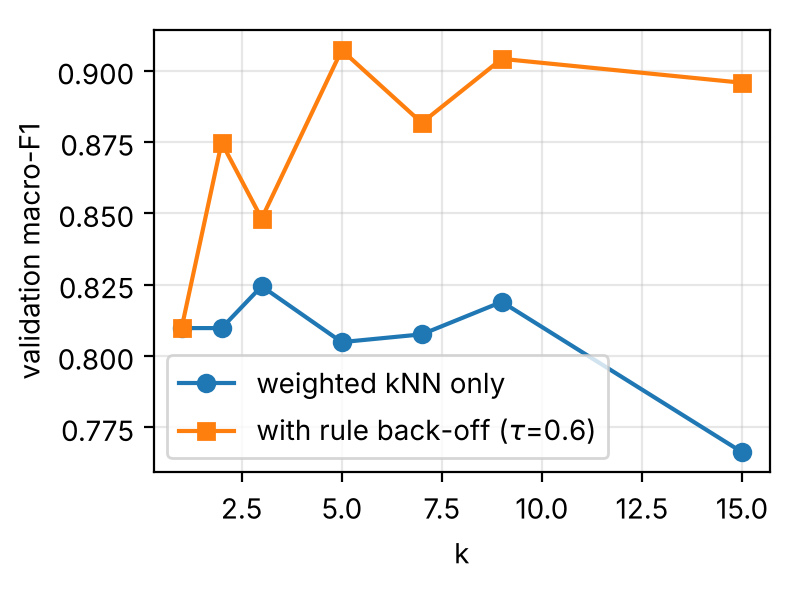
\includegraphics[width=0.9\linewidth]{../results/figures/tuning_k.png}
\caption{Validation macro-F1 for different $k$, with and without the rule back-off.}
\label{fig:tuning}
\end{figure}

\textbf{Tuning.} Figure~\ref{fig:tuning} shows validation macro-F1 against $k$. Without the rules, the best $k$ is 3 (0.824) and large $k$ gets worse, because more neighbours means the big classes \emph{earn} and \emph{acq} outvote the small ones. With the back-off ($\tau{=}0.6$) every $k>1$ improves, by between 0.02 and 0.13. $k{=}1$ cannot improve because with one neighbour the vote is always unanimous, so the rules are never used.

\begin{table}
\centering
\caption{Per-class test F1. N = number of test documents.}
\label{tab:perclass}
\setlength{\tabcolsep}{4pt}
\begin{tabular}{@{}lccccc@{}}
\toprule
Class & N & Rules & gzip & Ext. & SVM \\
\midrule
acq & 696 & 0.943 & 0.924 & 0.954 & 0.979 \\
crude & 121 & 0.871 & 0.841 & 0.905 & 0.967 \\
earn & 1083 & 0.966 & 0.965 & 0.979 & 0.992 \\
grain & 10 & 0.842 & 0.706 & 0.824 & 0.947 \\
interest & 81 & 0.724 & 0.747 & 0.844 & 0.886 \\
money-fx & 87 & 0.713 & 0.743 & 0.811 & 0.871 \\
ship & 36 & 0.880 & 0.635 & 0.787 & 0.896 \\
trade & 75 & 0.943 & 0.764 & 0.893 & 0.967 \\
\bottomrule
\end{tabular}
\end{table}

\begin{figure}[!htb]
\centering
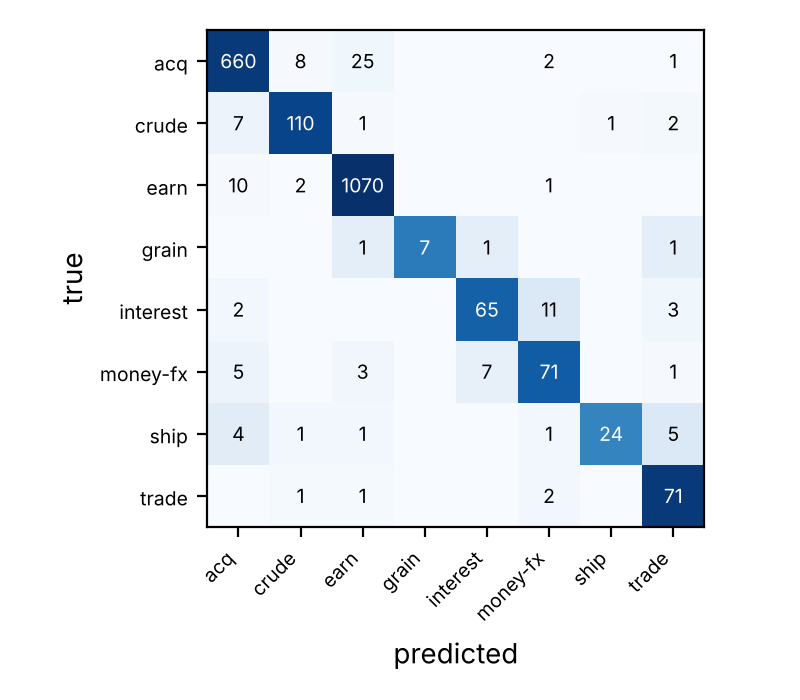
\includegraphics[width=0.85\linewidth]{../results/figures/confusion.png}
\caption{Confusion matrix of the extension on the test set (111 errors).}
\label{fig:cm}
\end{figure}

\textbf{Error analysis.} Table~\ref{tab:perclass} shows gzip is weakest on \emph{ship}, \emph{grain} and \emph{trade}, and the rules are much better on exactly these classes, which is why the back-off works. The extension improves on gzip for every class, but is still below the rules on \emph{grain}, \emph{ship} and \emph{trade}. Figure~\ref{fig:cm} shows the most common mistake is \emph{interest} vs \emph{money-fx} (18 of the 111 errors). These topics are very close: both are about central banks and money markets, and some of the labels look arguable. Many \emph{ship} errors are news about the Gulf war that were predicted as \emph{trade} or \emph{crude}, because they mention oil and Congress more than ships. Another error is a weather report for the ``Argentine grain belt'', which is mostly a table of place names. gzip finds that it looks like the earnings tables, and all the neighbours agree, so the rules are never asked even though they would get it right.

\section{Discussion}
\textbf{Comparison with the paper.} The paper reported gzip beating TF-IDF + logistic regression (0.954 vs 0.949). With fair scoring, gzip gets 0.916 and my tuned logistic regression gets 0.971, so the conclusion is reversed on R8. The paper's result depends on the top-2 scoring, and they also chose settings on the test set. My results agree with Opitz \cite{opitz2023}.

\textbf{Why the extension works.} gzip compares exact strings of characters, so two articles on the same topic with different wording look far apart, while articles that share boilerplate look close. The keyword rules look at topic words instead, so they make different mistakes. Using the rules only when the neighbours disagree combines the strengths of both. The weighted vote on its own did not help much, because a bigger neighbourhood is dominated by the large classes.

\textbf{Cost and interpretability.} gzip kNN has no training, but every prediction needs a compression against all 5,485 training documents, so it is much slower at test time than the SVM. The rules are fast and easy to explain, but they took manual work and would need updating for new topics.

\textbf{Limitations.} I only used one train/validation split, so I cannot say how much the results vary. For example, on the test set back-off with $k{=}2$ (0.882) is slightly better than the configuration chosen on validation (0.875). With only 10 \emph{grain} test documents, one document changes that class's recall by 0.1. I wrote the rules myself after looking at the training data, so another person might write different ones. I only tested gzip and one dataset.

\section{Conclusion}
I reproduced the gzip kNN result on R8 and showed that most of its advantage comes from the scoring method. Scored fairly, it is worse than a keyword classifier and TF-IDF models. Falling back to keyword rules when the neighbours disagree improved macro-F1 by about 0.08, but TF-IDF + linear SVM was still the best. In future work I would use several random splits to measure variance, try other datasets, and test whether the rules can also help a stronger model like the SVM.

\section*{USE OF AI TOOLS}
I used Claude minimally to proofread my coursework, mainly to
check grammar, spelling and sentence clarity. It supported my
learning by helping me identify areas where my writing could be
clearer and easier to understand. I reviewed all suggestions
carefully and only made changes that reflected my intended
meaning and writing style. I checked the revised text myself,
corrected any mistakes I identified and ensured that the
technical content, research, code, experiments and
conclusions remained my own work.
\bibliography{references}

\end{document}
